\documentclass[12pm,twosides,onecolumn,openany]{book}
\usepackage{graphicx} 
\usepackage[catalan]{babel}
\usepackage{emptypage}
\usepackage{hyperref}
\usepackage{mathtools}
\usepackage{blindtext}
\usepackage[utf8]{inputenc}
\usepackage{caption}
\usepackage{subcaption}
\usepackage{wrapfig}
\usepackage[a4paper]{geometry}
\geometry{top=2.5cm, bottom=2.5cm, left=2.5cm, right=2.5cm}
\usepackage{fancyhdr}
\pagestyle{fancy}
\usepackage{amsmath}
\usepackage{amssymb}
\usepackage{amsfonts}
\providecommand{\norm}[1]{\lVert#1\rVert}
\hypersetup{colorlinks=true,urlcolor=blue,linkcolor=blue}
\usepackage{multirow}
\usepackage{multicol}
\usepackage{rotating}
\usepackage{titlesec}
\usepackage{tcolorbox}
\usepackage{listings}
\usepackage{xcolor}

% Color de fons dels listings
\definecolor{bgcolor}{rgb}{0.94,0.94,0.94}

% Colors per a interpretar LaTeX al PDF
\definecolor{codegray}{rgb}{0.5,0.5,0.5}
\definecolor{codeblue}{rgb}{0,0,1}
\definecolor{codegreen}{rgb}{0,0.6,0}
\definecolor{codered}{rgb}{0.8,0,0}

% Configuració per a que listings entengui LaTeX
\lstdefinelanguage{LaTeX}{
    keywords={documentclass, usepackage, begin, end, chapter, section, subsection, textbf, textit, title, author, date, maketitle, tableofcontents, includegraphics, caption, label, ref, cite, pagestyle, thispagestyle, newpage, texttt, textsc, textsf},
    keywordstyle=\color{codeblue}\bfseries,
    morekeywords=[2]{include, input, newcommand, renewcommand, geometry, textcolor, footnote, emph},
    keywordstyle=[2]\color{codered}\bfseries,
    sensitive=true,
    comment=[l]{\%},
    morecomment=[s]{/*}{*/},
    commentstyle=\color{codegray}\itshape,
    string=[b]",
    stringstyle=\color{codegreen}
}

% Configuración global de la font per a listings
\lstset{
    language=LaTeX,
    basicstyle=\ttfamily\small,
    keywordstyle=\color{codeblue}\bfseries,
    backgroundcolor=\color{bgcolor},
    commentstyle=\color{codegray}\itshape,
    stringstyle=\color{codegreen},
    breaklines=true,
    breakindent=0pt,
    framexrightmargin=0.05\textwidth,
    linewidth=0.95\textwidth,
    frame=none,
    captionpos=b,
    numbers=left,
    numbersep=5pt,
    numberstyle=\tiny\color{gray},
    showspaces=false,
    showstringspaces=false,
    tabsize=4,
    inputencoding=utf8
}

\newenvironment{Figura}
  {\par\medskip\noindent\minipage{\linewidth}}
  {\endminipage\par\medskip}

\titleformat{\section}  % comando de sección a formatear
  {\fontsize{14}{16}\bfseries} % formato para toda la línea
  {\thesection} % cómo mostrar el número
  {0.4em} % espacio entre el número y el texto
  {} 
  [] 

% Comptador d'exemples
\newcounter{exemple}[section] 
\renewcommand{\theexemple}{\thechapter.\arabic{exemple}}
\newcommand{\exemple}[1]{
    \refstepcounter{exemple}
    \textbf{Exemple \theexemple} #1
}

% Configuració de la capçalera
\fancyhf{}
\fancyhead[RO,LE]{\rightmark}
\fancyhead[LO,RE]{\leftmark}
\fancyfoot[RO,LE]{\thepage}
\fancyfoot[LO,RE]{Curs d'Introducció a LaTeX}

\renewcommand{\chaptermark}[1]{\markboth{\thechapter.\ #1}{}}
\renewcommand{\sectionmark}[1]{\markright{\thesection.\ #1}}

\graphicspath{ {images/} }

\begin{document}
\newpage
\thispagestyle{empty}
\begin{titlepage}
    \centering
    \vspace*{\fill}  
    {\Huge \textsc{Curs d'Introducció a \LaTeX{}} \par}
    \vspace{1cm}
    {\Large Optica't UAB \par}
    \vspace{0.5cm}
    {\large Versió 1.0 \par}
    \vspace{5cm}
    \vspace*{\fill} 
\end{titlepage}


\newpage

\thispagestyle{empty}
Benvolguts i benvolgudes a aquest text introductori de LaTeX. Som Optica't, un grup de divulgació d'òptica física format per estudiants de la Universitat Autònoma de Barcelona. Aquest text està pensat per a facilitar l'aprenentatge d'aquesta eina a alumnes que comencin els seus estudis universitaris. Clarament, està orientat a graus científics, el nostre aprenentatge de LaTeX es basa en les necessitats i la curiositat que hem desenvolupat al llarg dels cursos en carreres com física o nanociències. Tot i això, pensem que LaTeX és una eina molt útil per a més disciplines i esperem que molta gent pugui fer profit d'aquest curs.

\newpage
\tableofcontents
\pagestyle{empty}
\newpage
Agraïments
\newpage
\pagestyle{fancy}
\chapter{Introducció i conceptes bàsics}
\thispagestyle{empty}

Dediquem aquest capítol a explicar des de zero com funciona LaTeX i com podem començar a crear els nostres primers documents. La finalitat del capítol és que us quedeu amb els conceptes bàsics de com funciona l'eina, la seva sintaxi, els possibles errors que trobareu, etc.

\section{Què és LaTeX i la seva utilitat}
LaTeX és un editor de textos que funciona de forma similar a un llenguatge de programació compilat. Està basat en el llenguatge de baix nivell \TeX{}, i està pensat principalment per a escriure textos científics de forma senzilla i elegant. La filosofia d'aquesta eina és que qui redacti no es preocupi del format del document, només en què ha d'escriure. A diferència d'un editor de textos \textsc{WYSIWYG} (en anglès, 'el que veus és el que obtens') al treballar amb LaTeX no podem veure el resultat del que redactem al moment d'escriure-ho. En LaTeX es treballa directament amb codi i després un compilador ho interpreta i genera un resultat (per exemple imprimeix el document per pantalla o genera un arxiu \texttt{.pdf}).\\\\
En un principi pot semblar que escriure en codi i no veure què és el que estem generant és contraproduent i pot fer menys atractiva la idea de treballar amb aquest editor i no amb altres més populars. Però, com veureu al llarg d'aquest text, aquest desavantatge queda opacat per la quantitat d'eines útils i de personalització que s'obtenen en treballar amb LaTeX.\\\\
Aquest curs se centra a abastar tot el necessari per a començar a escriure textos científics, com ara lliuraments de diverses assignatures de la carrera o per al treball de fi de grau. Però, en ser només un text introductori, no podrem explicar totes les eines que ofereix LaTeX bàsic i encara menys totes les eines que ha creat la comunitat. És necessari dir també que la utilitat d'aquest editor de textos va més enllà dels textos científics semblants a \textit{papers}. LaTeX té incorporades eines per a escriure llibres, per a escriure música, per a fer presentacions... Us convidem a informar-vos més enllà d'aquest text perquè podeu jugar amb totes les possibilitats que ofereix LaTeX tot i que no estudieu a cap branca científica.
\section{Entorns per a treballar amb LaTeX}
Per començar a treballar amb LaTeX primer necessitem saber on! És a dir, necessitem saber quin és el nostre entorn de treball. Igual que passa amb els llenguatges de programació, podem córrer LaTeX a dins d'una gran varietat d'entorns. Cada entorn és lleugerament diferent de l'altre, les seves característiques depenen de la versió i de quin sigui el flux de treball pensat específicament per a aquell entorn. Escollir un bon entorn pot arribar a ser una mica enrevessat, per tant, per a facilitar la tasca a les persones que encara no han fet servir LaTeX o que no estiguin familiaritzades en treballar amb programes de manera local centrarem el curs en l'entorn d'Overleaf. Sense ser exhaustius també parlarem sobre altres entorns com algunes eines d'escriptori o a escriure directament en un document de text amb eines més específiques de programació.\\\\
Per al lector o lectora que ja tingui experiència amb Overleaf i vulgui fer servir les altres eines, pròximament crearem una guia que complementi aquest curs amb més informació, de moment ens centrarem en que pugueu escriure el vostre primer document en LaTeX.
\subsection{Overleaf}
L'entorn per exce\lgem ència per a aprendre LaTeX i per a fer petits projectes co\lgem aboratius és Overleaf. Per a fer-ho servir no cal insta\lgem ar-se res, només necessites connexió a internet i un usuari. Overleaf és un entorn de LaTeX en línia pensat per a fer més fàcil la co\lgem aboració entre usuaris a l'hora de crear un document compartit. Els seus avantatges són:
\begin{itemize}
    \item No requereix cap insta\lgem ació, només tenir un compte. Per a poder accedir a un compte d'Overleaf només necessiteu un correu electrònic i entrar a la web oficial\footnote{Us deixem l'enllaç vigent actualment: \url{https://es.overleaf.com}}

    \item Interpreta el codi fins i tot si aquest conté algun petit error

    \item Permet treballar conjuntament amb diverses persones\footnote{Actualment (inici del 2025) la limitació per a editar el mateix projecte d'Overleaf es limita a dos usuaris. La resta d'usuaris que entrin al projecte només poden llegir-ho.}

    \item Permet classificar els teus projectes amb etiquetes

    \item Té insta\lgem ats alguns paquets que el LaTeX pur no té per defecte

    \item Té un sistema de navegació i una visualització del log de compilació intuïtius 

    \item Té integrades algunes eines que faciliten la generació de codi, com ara botons o \textit{short cuts} que canvien el format del text com en Word o un generador de taules buides

    \item Proporciona un editor visual on es pot treballar en un entorn semblant a un editor WYSIWYG
\end{itemize}
Com aquesta serà l'eina que farem servir a la resta del curs, explicarem una mica més sobre com funciona. Un cop tinguem obert un compte podrem crear un nou projecte des del menú principal. Overleaf ofereix moltes plantilles preestablertes, però per a aprendre treballarem amb una plantilla buida. Un cop obert el nou projecte en blanc veurem la següent pantalla:

\begin{figure}[h]
    \centering
    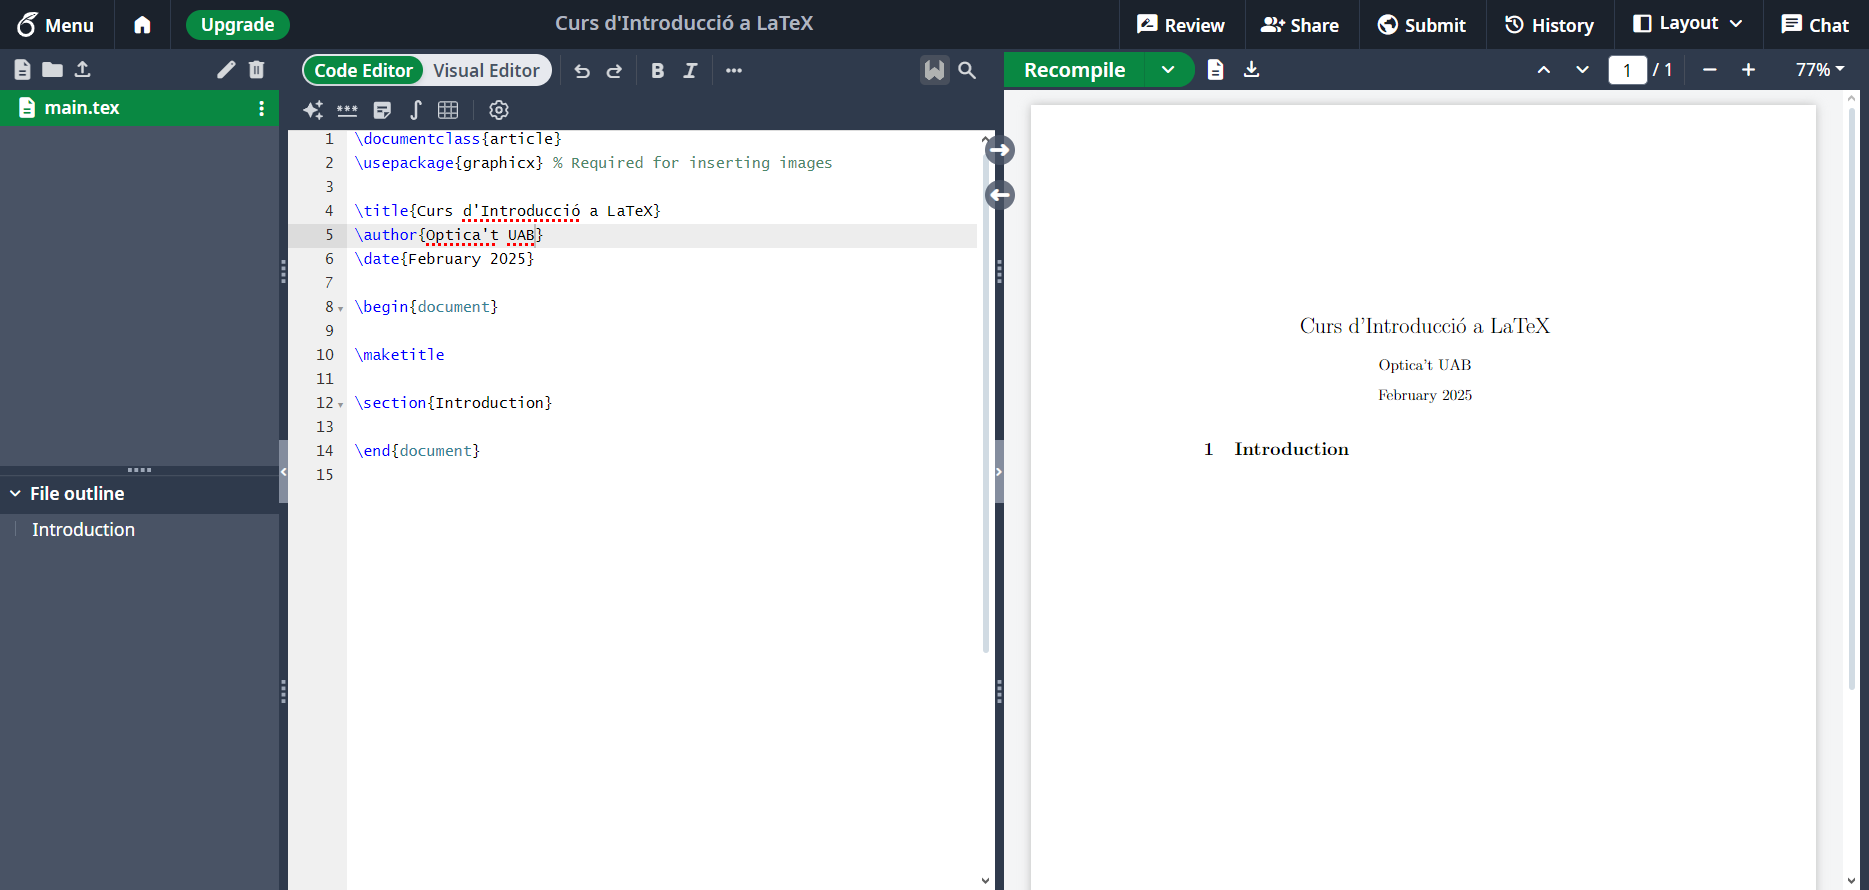
\includegraphics[width=0.95\linewidth]{../Text principal/Imatges/captura_nou_projecte.png}
    \caption{Entorn de treball d'Overleaf per a un projecte en blanc.}\label{fig:entorn_Ovlf_blanc}
\end{figure}

\noindent Observem de la Figura \ref{fig:entorn_Ovlf_blanc} que l'entorn se separa en tres parts. A l'esquerra del tot observem un menú, l'explorador d'arxius i de projecte. Aquest explorador funciona com a un gestor de carpetes i d'arxius, molt similar a l'explorador d'arxius de Windows. A la part superior de l'explorador aniran apareixent els arxius que fem servir al projecte. Podem mantenir un ordre d'aquests arxius utilitzant carpetes i canviant el nom de cada arxiu com vulguem. A la part inferior de l'explorador apareixerà un llistat de títols que ens serveixen per a moure'ns pel projecte de forma més senzilla, expliquem el seu funcionament amb més detall a la secció \ref{sec:cap_sec_subsec}.\\\\
A la dreta de la pantalla s'observa un visor pdf. Aquest visor permet veure per pantalla com va quedant el document que estem generant amb el codi que hem escrit. Notareu que a la part superior esquerra del visor hi ha un botó verd on posa \texttt{Recompile}. Cada cop que vulguem actualitzar el pdf amb la informació que hem escrit en codi hem de fer click a \texttt{Recompile}\footnote{No cal fer click sempre, existeixen dues alternatives. La primera és fer servir \textit{short cuts}, és a dir, prémer \texttt{Ctrl + s} o bé \texttt{Ctrl + Enter}. La segona és activar la funció automàtica de recompilat. Podeu accedir a aquesta opció desde el botó \texttt{Recompile}, prement la fletxa que té al costat.}. Diem a aquesta acció recompilar o compilar el codi.\\\\
Entre l'explorador i el visor tenim l'editor de text. Aquest editor és igual que qualsevol altre en programació. Allà és on escrivim totes les línies de codi necessàries per a generar el nostre document. Tot i això, aquesta finestra intermitja no sempre farà d'editor. Overleaf permet treballar amb més tipus d'arxiu que els de LateX com per exemple imatges. Per tant és més encertat pensar en l'editor com un entorn dinàmic de treball i no només com un simple editor de text.\\\\
Es pot configurar la visibilitat tant de l'editor com del visor pdf a partir de les opciones del desplegable \texttt{Layout}. Aquestes opcions deixen només visible un dels dos, els dos o permet separar-los en finestres diferents del navegador (això és útil si per exemple treballem a doble pantalla).
\subsection{LaTeX d'escriptori}
Aquí va el text que redactarà Aurem :)
\subsection{Eines alternatives}
Per a la gent més experimentada o amb més interés en la programació deixem el següent entorn que, tot i potser semblar més complicat de fer servir, permet personalitzar completament el teu entorn de treball. LaTeX és un llenguatge, no un programa, per tant desde qualsevol editor de text podem escriure en LaTeX i, fent servir el compilador corresponent podrem generar la sortida que vulguem. Ara bé, existeixen eines que faciliten aquesta feina i ens permeten configurar el nostre entorn de forma més visual. Podriem fer una llista enorme amb eines de visualització útils i personalitzables, però una de les més populars (i des de la que s'està redactant aquest text) és Visual Studio Code. La instalació i configuració d'aquest entorn queda fora dels proposits d'aquest curs, però us convidem a informar-vos una mica sobre aquesta eina ja que no serveix només per a LaTeX. Visual Studio Code permet treballar amb LaTeX (i molts més llenguatges) en local, té integrat un explorador de directoris molt visual (no cal barallar-se amb la bash per a navegar per les carpetes) i permet afegir extensions pensades per a treballar amb LaTeX.
\section{Estructura bàsica d'un document}
De forma similar a un llenguatge de programació quan escrivim un document en LaTeX necessitem seguir un cert ordre i respetar una sintaxi concreta per a que el compilador pugui comprendre i traduïr correctament el nostre document. Aquestes normes que s'han de seguir no són complicades, de fet amb Overleaf són similars a escriure en Word. Com hem comentat abans, LaTeX està pensat per a que no ens haguem de preocupar per la forma sinó més per qué escrivim, per tant és aquí on hi ha la diferència principal amb altres eines d'edició de textos. 
\subsection{Sintaxi}
L'estructura d'un document de LaTeX se separa en dues parts ben diferenciades:
\begin{itemize}
    \item \textbf{Preàmbul}: a on escrivim la ``configuració'' del document
    \item \textbf{Text principal}: a on escrivim el cos del document
\end{itemize}
Separem aquestes dues parts de forma explícita, reservant sempre les primeres línies de codi per al preàmbul i la resta per al text principal. Veiem com a exemple el codi que escriu Overleaf per defecte quan obrim un document en blanc:\\\\
\exemple{\label{ex:\theexemple}}\footnote{Tant Overleaf com LaTeX permet fer servir accents escrits directament amb el teclat o amb codi (ho veurem més endavant). Però, l'entorn que fem servir per a escriure els exemples no els detecta correctament. Això no serà un problema per a volsaltres a l'hora de redactar un document sense aquest recurs. Si us plau, feu servir accents.}
\begin{lstlisting}
    \documentclass{article}
    \usepackage{graphicx} % Required for inserting images

    \title{Curs d'Introduccio a LaTeX}
    \author{Optica't UAB}
    \date{February 2025}

    \begin{document}

    \maketitle

    \section{Introduction}

    \end{document}
\end{lstlisting}
Des de la primera línia fins a la setena és el preàmbul. La resta és el text principal i comença amb el comandament \texttt{\textbackslash begin\{document\}}. 
L'exemple \ref{ex:1.1} ens permet veure els tres tipus de comandaments bàsics del preàmbul i com s'estructura un document. El preàmbul de l'exemple comença declarant a la primera línia el tipus de document que estem redactant. Seguidament, a la segona, declara el paquet \texttt{graphicx}. Els últims tres comandaments configuren tres objectes predefinits (el títol, l'autor i la data). Veiem doncs que al preàmbul els comandaments bàsics que podem fer servir són:
\begin{itemize}
    \item[-] Declaració de tipus de document
    \item[-] Declaració de paquets
    \item[-] Configuració d'entorns pre-establerts
\end{itemize}
Parlarem amb més detall d'aquests comandaments a les següents seccions (\ref{sec:tipus_de_document}, \ref{sec:paquets} i \ref{sec:entorns}). La resta del document, alló que es plasmarà al compilar, es redacta en un entorn delimitat pels comandaments \texttt{\textbackslash begin\{document\}} i \texttt{\textbackslash end\{document\}}. El codi que hi ha escrit entre aquests delimitadors serveix per a imprimir al document el títol i el títol de la secció anomenada ``Introduction''. Més endavant ens interessarem per aquests comandaments. Encara més important per a aquesta part del codi és com es redacta text pla per a que s'imprimeixi com volem per pantalla. Veiem-ne alguns exemples:\\\\
\exemple{\label{ex:\theexemple}}
\begin{lstlisting}
    \documentclass{article}

    \begin{document}
        Aixo s'escriu en text pla, amb una mida de font standar i amb 
        uns marges per defecte.
    \end{document}
\end{lstlisting}
\textbf{Sortida:}
\begin{tcolorbox}[colframe=black, colback=white, sharp corners, width=\textwidth,boxrule=0.2mm]
    Aixo s'escriu en text pla, amb una mida de font standar i amb uns marges per defecte.
\end{tcolorbox}
Com veiem el text s'escriu justificat a l'amplada del document i amb una mida de text normal. La mida i el tippus de lletra es pot modificar tant a la configuració del preàmbul com al mateix codi (veure secció \ref{sec:format_del_text_pla}). Si tenim més text aquest s'adaptarà en forma de paràgraf. Existeixen diverses formes de separar dos paràgrafs i cada forma crea un salt de línia de diferent mida i genera o no indentació per defecte.\\\\
\exemple{\label{ex:\theexemple}}
\begin{lstlisting}
    \documentclass{article}

    \begin{document}
        Aquest es un text d'exemple que omplira l'amplada del document formant un unic paragraf. Podem separar-ho en altres paragrafs de diferents maneres.\\
        Aquest paragraf esta separat per $\backslash\backslash$. S'aplica un salt de linia normal, amb una separacio igual a la d'un salt de linia del mateix paragraf i no aplica indentacio.

        Deixar una linia en blanc tambe genera un altre paragraf com al escriure $\backslash\backslash$ pero a mes aplica indentacio. Si LaTeX detecta que hi ha mes d'un espai en blanc normalment avisa amb un error de sintaxi. Overleaf permet fer aquest espais en blanc i ho interpreta com a un de sol.Podem generar el mateix efecte separant el paragraf amb el comandament $\backslash$par. LaTeX quan es troba aquest comandament enten que s'ha acabat un paragraf i que lo que ve a continuacio pertany a un seguent paragraf. \par Per exemple aquest text esta separat pel comantament $\backslash$par.\\\\
        Aquest darrer paragraf se separa amb quatre $\backslash$. Aquesta forma de separar paragrafs no genera indentacio i crea un salt de linia mes gran, fent que el text se separi en dos de forma mes visual. 
    \end{document}
\end{lstlisting}
\textbf{Sortida:}
\begin{tcolorbox}[colframe=black, colback=white, sharp corners, width=\textwidth,boxrule=0.2mm,parbox=false]
    Aquest es un text d'exemple que omplira l'amplada del document formant un unic paragraf. Podem separar-ho en altres paragrafs de diferents maneres.\\
    Aquest paragraf esta separat per $\backslash\backslash$. S'aplica un salt de linia normal, amb una separacio igual a la d'un salt de linia del mateix paragraf i no aplica indentacio.

    Deixar una linia en blanc tambe genera un altre paragraf com al escriure $\backslash\backslash$ pero a mes aplica indentacio. Si LaTeX detecta que hi ha mes d'un espai en blanc normalment avisa amb un error de sintaxi. Overleaf permet fer aquest espais en blanc i ho interpreta com a un de sol.Podem generar el mateix efecte separant el paragraf amb el comandament $\backslash$par. LaTeX quan es troba aquest comandament enten que s'ha acabat un paragraf i que lo que ve a continuacio pertany a un seguent paragraf. \par Per exemple aquest text esta separat pel comantament $\backslash$par.\\\\
    Aquest darrer paragraf se separa amb quatre $\backslash$. Aquesta forma de separar paragrafs no genera indentacio i crea un salt de linia mes gran, fent que el text se separi en dos de forma mes visual. 
\end{tcolorbox}

El detall de com escriure $\backslash$ dins del codi per a que s'imprimeixi correctament ho explicarem més endavant. A l'exemple \ref{ex:1.3} podem veure quatre formes de separar paràgrafs. L'ús d'un salt o altre ve a gust de qui està redactant el document. En aquest text, per exemple, normalment separem els paragrafs amb $\backslash\backslash\backslash\backslash$ per a obtenir un efecte visual més polit. La separació de paràgrafs de vegades ve condicionada pel que té el paràgraf al seu voltant, usualment pel codi just a sobre d'ell\footnote{Això ho veureu a mesura que escriviu documents en LaTeX, lo més usual és veure-ho quan es comença un paràgraf després de posar una figura o una taula. Per exemple, al finalitzar l'exemple \ref{ex:1.3} comença un paràgraf amb indentació automàtica.}. En cas de voler afegir o treure una indentació desitjada o no podem fer servir el comandament $\backslash$\texttt{indent} o $\backslash$\texttt{noindent}.\\\\
La indentació a LaTeX pot portar una mica de confusió no només amb el que s'imprimeix en pantalla al genrar el resultat, sinó també amb la indentació dins del propi codi. L'estructura del codi que escrivim ve imposada pel fet que hem de fer entendre al compilador què volem que surti exactament. Però, per a poder facilitar la nostra lectura del codi podem fer servir una jerarquia amb la indentació dins del codi. Fixem-nos novament en l'exemple \ref{ex:1.3}, el text que s'acabarà imprimint al document es troba indentat respecte als delimitadors del document (el \texttt{begin} i el \texttt{end}). Podriem escriure aquest codi sense aplicar aquesta indentació i el resultat per pantalla acabaria sent el mateix que abans. Aquesta indentació global el compilador la ignora, però a nosaltres ens és útil per a saber que aquella part del codi pertany al document. En cas de ternir més entorns a dins del codi (com veurem a la secció \ref{sec:entorns}) podem aprofitar aquesta indentació per a poder escriure un codi més polit que pugui ser fàcilment entés tant pel compilador com per a qui escriu o revisa el codi.
\subsubsection{Paraules reservades i comandaments}
Com heu pogut observar als exemples que hem posat fins ara hi ha algunes paraules que les hem posat en color blau. Semblant a un llenguatge de programació, LaTeX té un conjunt de paraules i simbols reservats per a que el compilador entengui si estem escrivint text pla o si estem donant una ordre concreta. Els comandaments (ja siguin del preàmbul o a dins del text o entorns matemàtics) venen declarats començant pel símbol ``$\backslash$''\footnote{És per aquest motiu que no hem escrit directament el símbol al codi per a que s'imprimeixi en la sortida del document, ja que LaTeX ho interpretaria com a un comandament i no com a un símbol}. Entorns visuals com Overleaf faciliten la tasca de saber quines són aquestes paraules reservades canviant el seu color al codi o fins i tot fent prediccions del codi que volem escriure.\\\\
No és viable aprendre de forma activa quines són aquestes paraules (no recomenem provar-ho, és una tasca molt farragosa). Lo més útil és practicar i amb el temps acostumar-se a la forma intuituva que té LaTeX de seleccionar aquestes paraules, ja que normalment són instruccions literals en anglès. Al llarg del curs explicarem algunes d'aquestes paraules reservades i a l'Annex deixarem algunes taules amb exemples útils que podeu fer servir al vostre dia a dia.\\\\
A més, veureu que acompanyant a aquestes paraules reservades normalment apareixen \{ \} o [ ]. Entre claus normalment s'escriu l'argument de la funció que estiguem cridant amb la paraula reservada. Entre claudators normalment s'escriuen les opcions de configuració de la funció.
\subsection{Tipus de document}\label{sec:tipus_de_document}
Fixem-nos ara en la primera línia del preàmbul. Com hem dit aquest comandament declara quin tipus de document estem escrivint. Segons com configurem aquesta línia, el text que redactem sortirà amb una configuració predefinida o altre. Aquesta configuració és molt bàsica, però pot portar a problemes que semblen que no tenen solució si no es té en compte qué hem configurat i que no. Existeixen molts tipus de documents que enten LaTeX, comentem per sobre els més comuns:
\begin{itemize}
    \item \textbf{\texttt{article}} - Aquest és el tipus de document que normalment fareu servir a la carrera. Està pensat per a escriure documents científics curts, de forma que permet estructurar el text en seccions.
    \item \textbf{\texttt{report}} - En cas de necessitar fer un article més llarg podeu fer servir aquest tipus de document. Un \texttt{report} permet a més de seccions separar el text en capítols.
    \item \textbf{\texttt{book}} - Aquest és el tipus de document que fem servir per a redactar aquest curs. Treballa de forma similar a un report (és un text llarg i amb capítols) pero afegeix detalls necessaris per a estructurar un llibre. Un exemple molt clar d'això és que de forma automàtica genera l'espai en blanc adient per a que els capítols començin en una pàgina imparella.
    \item \textbf{\texttt{letter}} - En cas de voler escriure una carta amb una estructura formal podeu fer servir aquesta classe de document. \texttt{letter} permet declarar al preàmbul algunes variables predefinides (com la signatura o l'acomiadament) que serveixen per a estructurar la carta de forma molt senzilla.
    \item \textbf{\texttt{beamer}} - Aquest darrer format serveix per a crear presentacions. És una classe de document molt personalitzable, però és més complicada de fer servir i això la fa una mica limitada per a la gent que comença a fer servir LaTeX.
\end{itemize}

Cada classe de document es pot configurar com més ens convingui. L'estructura del comandament sencer és $\backslash$\texttt{documentclass[...]\{\textit{class}\}} on entre claudators podem escriure la configuració i entre claus la classe de document que vulguem. Les configuracions poden ser molt variades i es pot posar més d'una entre els claudators sempre que les separem per comes. Deixem algunes configuracions comunes amb una breu explicació i alguns exemples:
\begin{itemize}
    \item Es pot modificar la mida de la lletra del text pla general posant \texttt{10pm}, \texttt{11pm}, \texttt{12pm}, etc. La unitat de mesura \texttt{pm} s'anomena punt i correspon a aproximadament 0,35$\,$mm al paper.
    \item Podem configurar la mida del paper segons desitjem. Per defecte en un document \texttt{book} la mida és A4, però en altres pot variar. Podem explicitar diferents mides com \texttt{a4paper} (mida A4), \texttt{letterpaper} (mida de carta, 216 $\times$ 279$\,$mm), \texttt{b5paper} (format B5, 176 $\times$ 250$\,$mm), etc. 
    \item Configurem el format d'impressió a una o doble cara, amb els comandaments \texttt{oneside} i \texttt{twoside} respectivament. Aquesta configuració canvia per exemple quan comença un capítol, si a la següent pàgina o a la següent pàgina imparella. Cada configuració està pensada per a que es pugui enquadernar a una o a dues cares.
    \item Configurem la distribució del text ja sigui a una o a doble columna\footnote{Això configura el text de forma general, tot el text s'estructurarà en una a dues columnes. Per a obtenir una millor personalització de la doble columna farem servir altres comandaments (veure secció \ref{sec:multiples_columnes}).} amb els comandaments \texttt{onecolumn} per a una columna i \texttt{twocolumn} per a dues.
    \item Podem escollir si els capítols comencen a qualsevol pàgina (\texttt{openany}) o a les pàgines imparelles (\texttt{openright}).
\end{itemize}
\exemple{\label{ex:\theexemple}} \textbf{Article en format A4 amb lletra de mida 10pm:}
\begin{lstlisting}
    \documentclass[10pm]{article}
\end{lstlisting}
\exemple{\label{ex:\theexemple}} \textbf{Report mida A4, a dues columnes, lletra mida 12pm i a una cara:}
\begin{lstlisting}
    \documentclass[a4paper,12pm,oneside,twocolumn]{report}
\end{lstlisting} 
\exemple{\label{ex:\theexemple}} \textbf{Configuració d'aquest document:}
\begin{lstlisting}
    \documentclass[12pm,twosides,onecolumn,openany]{book}
\end{lstlisting}

Veiem a l'exemple \ref{ex:1.6} que hem aplicat \texttt{openany} i no hem explicitat \texttt{a4paper} (no és necessari, \texttt{book} ho té onfigurat per defecte). Això es deu a que aquest document està escrit per a llegir-se en format digital i no en paper. La versió en paper d'aquest document no hauria d'escriure l'opció \texttt{openany} i deixar per defecte \texttt{openright} (es podria escriure explícitament, però \texttt{book} té aquesta darrera opció per defecte).
\subsection{Paquets}\label{sec:paquets}
Com hem dit existeixen molts comandaments que podem escriure a partir de paraules reservades. Amb aquests comandaments podem, com si fos un llenguatge de programació, configurar funcions que ens modifiquen el que imprimim per defecte en un document escrit en LateX. Però, aquesta tasca és molt farragosa, ja que per a fer servir eines molt comunes hauriem de saber la configuració exacta de cada detall que necessitem escriure. És per això que, novament com als llenguatges de programació, existeixen els paquets. Aquests paquets són codi en LaTeX escrit per a configurar diverses funcions que necessitem per a redactar, hi ha molts i de molt diferents. Alguns venen per defecte amb LaTeX i altres venen per part de la comunitat. El funcionament de cada paquet és molt diferent a cada un, fins i tot podem trobar alguns obsolets o incompatibles entre ells. Però, de forma senzilla podem explicar el seu funcionament dient que són comandaments que indiquen a LaTeX que existeixen noves paraules reservades preconfigurades.\\\\
Per a poder fer servir un paquet hem de cridar-lo explícitament al preàmbul amb el comandament $\backslash$\texttt{usepackage\{...\}}, just després de declarar el tipus de document. Podeu trobar paquets molt interessants buscant per internet, us deixem un breu llistat amb alguns exemples:
\begin{itemize}
    \item $\backslash$\texttt{usepackage[a4paper]\{geometry\}} - Aquest paquet és útil per a configurar els marges del document, aquest exemple adapta els d'un de mida A4.
    \item $\backslash$\texttt{usepackage\{caption\}} - Permet configurar la lletra dels títols de taula i peus de figura.
    \item $\backslash$\texttt{usepackage\{fancyhdr\}} - Serveix per a configurar la capçalera i els peus de pàgina.
    \item $\backslash$\texttt{usepackage\{mhchem\}} - Permet escriure més fàcilment fòrmules i reaccions químiques.
\end{itemize}

Fent referència a l'explicació simplificada de lo que és un paquet podem veure l'exemple de \texttt{mhchem}. Aquest paquet indica a LaTeX que existeix una nova paraula reservada assignada al comandament ``$\backslash$\texttt{ce}\{...\}'' la qual amb els arguments adients ens permet escriure fòrmules o reaccions químiques més fàcilment.\\\\
Un detall important a l'hora d'utilitzar paquets és que no tots es troben insta\lgem ats per defecte a LaTeX. Això depèn molt de l'entorn on es treballi, pot variar fins i tot segons la versió o la distribució que us hagueu insta\lgem at en local. Overleaf té l'avantatge que la majoria de paquets útils ja venen insta\lgem ats i no us haureu de preocupar per això\footnote{Per exemple, \texttt{mhchem} es pot fer servir a Overleaf sense cap problema, però en local s'ha d'insta\lgem ar prèviament.}. La resta d'usuaris que no feu servir Overleaf haureu d'insta\lgem ar els paquets que no tingueu per defecte segons quin entorn estigueu fent servir, ja sigui des de la web dels creadors del paquet o directament llençant un comandament des de la bash en Windows o Linux.\\\\
El funcionament de cada paquet es pot trobar a internet, normalment es pot trobar a la bibliografia oficial del paquet o es pot demanar ajuda a eines d'inte\lgem igència artificial per a que us donin alguna breu explicació. En aquest curs farem servir i explicarem com funcionen diversos paquets comuns o útils.
\subsection{Entorns}\label{sec:entorns}
Posem novament enfasi a les paraules reservades. Com hem dit anteriorment el codi que s'acabarà imprimint al document es troba entre els delimitadors $\backslash$\texttt{begin\{document\}} i $\backslash$\texttt{end\{document\}}. Les paraules clau \texttt{begin} i\texttt{end} són dues paraules reservades molt comunes en un codi de LaTeX, ja que obren i tanquen entorns específics dins del codi. Els arguments que accepten aquests delimitadors poden ser molt diversos, de fet podem obtenir nous arguments afegint paquets. L'ús de delimitadors per a construïr entorns és molt útil tant per a accedir a les funcions que necessitem per a escriure el nostre text com per a seguir una jerarquia al codi (com vam dir al parlar de la sintaxi). Ja sigui indentat o no, el codi que es troba entre els delimitadors constitueix un bloc aïllat de la resta del codi. Qualsevol comandament (llevat d'aquells que actuen globalment) que escrivim dins de l'entorn delimitat només afectarà al codi que hi hagi dins.\\\\ 
Exemples d'entorns propis de LaTeX són l'entorn matemàtic (parlem més profundament al capítol \ref{cap:entorn_matematic}), \texttt{equation}; l'entorn de justificació central, \texttt{center}; l'entorn de justificació cap a la dreta, \texttt{flushright}; l'entorn de les figures, \texttt{figure}; etc. Exemples d'entorns  d'alguns paquets són: ambl el paquet \texttt{subcaption} l'entorn de les subfigures, \texttt{subfigure}; amb el paquet \texttt{tcolorbox} l'entorn d'un quadre de text amb marcs i fons configurable, \texttt{tcolorbox}; amb el paquet \texttt{listings}  l'entorn que permet escriure amb diferent format que el text normal codi en altre llenguatge de programació, \texttt{lstlisting}, etc. Aquests últims exemples necessiten primer una configuració extra al preàmbul, per tant són una mica més avançats que la resta d'entorns que venen per defecte amb LaTeX. Podeu veure com es fan servir aquests entorns al següent exemple:\\\\
\exemple{\label{ex:\theexemple}}
\begin{lstlisting}
    \documentclass{article}
    
    \usepackage{subcaption}
    \usepackage{listings}
    \usepackage{tcolorbox}

    \begin{document}
        Aquest text esta justificat per defecte ja que no es troba dins de cap entorn, nomes es troba dins del document.\\

        \begin{center}
            El text que es troba aqui esta justificat al centre. S'observa com per a poder veure millor el codi fem servir indentacio, pero com hem dit el compilador omet aquesta indentacio global. Tambe es veu com separem en paragrafs. La combinacio d'espai en blanc i $\backslash\backslash$ es equivalent a quatre $\backslash$.
        \end{center}

        \noindent Parlarem mes endavant, pero podeu veure un exemple matematic:

        \begin{equation*}
            a^2 + b^2 = c^2
        \end{equation*}

        \begin{flushright}
            Podem tambe escriure text justificat cap a la dreta. Qualsevol objecte dins d'aquet entorn que no tingui una justificacio fixa es justificara cap a la dreta juntament amb el text. Un exemple d'aixo pot ser una imatge.
        \end{flushright}

        \begin{tcolorbox}[colframe=red, colback=black!5!white, sharp corners, width=0.85\textwidth,boxrule=0.2mm,parbox=false]
            Aquest text te justificacio per defecte pero envoltat per una caixa. La configuracio explicita dels colors i la mida es troba entre claudators. La configuracio implicita es troba en el preambul del document del curs, parlarem mes endavant d'allo.
        \end{tcolorbox}
    \end{document}
\end{lstlisting}
\textbf{Sortida:}
\begin{tcolorbox}[colframe=black, colback=white, sharp corners, width=\textwidth,boxrule=0.2mm,parbox=false]
    Aquest text esta justificat per defecte ja que no es troba dins de cap entorn, nomes es troba dins del document.\\

    \begin{center}
        El text que es troba aqui esta justificat al centre. S'observa com per a poder veure millor el codi fem servir indentacio, pero com hem dit el compilador omet aquesta indentacio global. Tambe es veu com separem en paragrafs. La combinacio d'espai en blanc i $\backslash\backslash$ es equivalent a quatre $\backslash$.
    \end{center}

    \noindent Parlarem mes endavant, pero podeu veure un exemple matematic:

    \begin{equation*}
        a^2 + b^2 = c^2
    \end{equation*}

    \begin{flushright}
        Podem tambe escriure text justificat cap a la dreta. Qualsevol objecte dins d'aquet entorn que no tingui una justificacio fixa es justificara cap a la dreta juntament amb el text. Un exemple d'aixo pot ser una imatge.
    \end{flushright}

    \begin{tcolorbox}[colframe=red, colback=black!5!white, sharp corners, width=\textwidth,boxrule=0.2mm,parbox=false]
        Aquest text te justificacio per defecte pero envoltat per una caixa. La configuracio explicita dels colors i la mida es troba entre claudators. La configuracio implicita es troba en el preambul del document del curs, parlarem mes endavant d'allo.
    \end{tcolorbox}
\end{tcolorbox}

Veiem a l'exemple \ref{ex:1.7} com fem sesrvir alguns dels entorns que hem emncionat abans. Els detalls del funcionament de cada un ho veure deprés, de moment quedeu-vos amb com es treballa amb els entorns.\\\\
Aquesta forma de treballar és essencial, ja que ens permet fer servir comandaments locals que afecten a tot el codi que es trobi dins d'un entorn. Per exemple, existeix el comandament \texttt{centering}. Aquest és un comandament local, que afecta a tot el seu entorn fins a trobar uns delimitadors (si no hi ha un entorn escrit, els delimitadors són els del mateix \texttt{document}). El comandament \texttt{centering} justifica al centre el tot a tot alló que es trobi en el seu entorn. Si és text lo que hi ha dins d'aquest entorn, \texttt{centering} funciona igual que l'entorn \texttt{center}.

\chapter{Format de text i estructura}
Aquest capítol del curs el dedicarem a aprendre a construir documents de LaTeX amb les eines més senzilles d'edició del format del text que en permet LaTeX pur. Veureu que els diferents apartats són, bàsicament, una recopilació dels comandamens més comuns que es fans servir per a redactar la majoria de textos científics amb aquesta eina.
\thispagestyle{empty}
\section{Format del text pla}\label{sec:format_del_text_pla}
Al capítol anterior hem vist com funciona la sintaxi del text pla, com podem separar-lo per paràgrafs i com fer servir paquets i entorns útils que ens són de molta utilitat per a poder redactar documents interessants. Ara parlarem de certs comandaments, també molt bàsics, que permeten configurar el tipus de lletra que fem servir.\\\\
Hi ha molts comandaments, ja siguin integrats a LaTeX o que provenen de paquets que ens modifiquen la font del text pla que redactem. Tots aquests comandaments funcionen de la mateixa forma: el text afectat ha de ser l'argument del comandament. Podem fer una breu classificació d'aquests comandaments amb alguns exemples que us deuxem a continuació.
\subsubsection{Modificacions comunes}
\begin{center}
    $\backslash$\texttt{textbf}\{Text en negreta\} \textbf{Text en negreta} \hspace{1.5cm} $\backslash$\texttt{textit}\{Text en cursiva\} \textit{Text en cursiva}\\ \vspace{5mm}
    $\backslash$\texttt{underline}\{Text subratllat\} \underline{Text subratllat}
\end{center}
\subsubsection{Tipus de font}
\begin{center}
    $\backslash$\texttt{text}\{Text normal\}\footnote{Aquest comandament i un altre ens serà útil en entorns matemàtics. Per escriure text pla normal no cal fer-lo servir.} \text{Text normal} \hspace{1.5cm} $\backslash$\texttt{textsf}\{Text en Sans Serif\} \textsf{Text en Sans Serif}\\ \vspace{5mm}
    $\backslash$\texttt{texttt}\{Text mecanografiat\} \texttt{Text mecanografiat} \\ \vspace{0.5cm} $\backslash$\texttt{textsc}\{Text en majúscules petites\} \textsc{Text en majúscules petites}
\end{center}
Per a fer canvis en la mida de la lletra fem servir uns comandaments locals que afecten tot l'entorn on treballem. Tan com si escribim en un entorn concret d'alguna funció com si escrivim text pla podem delimitar la part del codi a la que afecten aquests comandaments fent servir claus com a delimitadors. Un exemple general (i inventat) d'aquesta sintaxi per als comandaments locals és: 
\begin{center}
    \{$\backslash$\texttt{comandament} Aquest text està afectat pel comandament exemple\}.
\end{center}
Posem a continuació alguns exemples de mida de lletra.
\subsubsection{Mida de lletra}
\begin{center}
    \{$\backslash$\texttt{tiny} Text tiny\} {\tiny Text tiny} \hspace{1cm} \{$\backslash$\texttt{footnotesize} Text de footnote\} {\footnotesize Text de footnote} \\ \vspace{5mm}  \{$\backslash$\texttt{large} Text large\} {\large Text large} \hspace{1cm}  \{$\backslash$\texttt{huge} Text huge\} {\huge Text huge}
\end{center}
Podeu trobar més exemples i el llistat complet de mides a l'Annex. Naturalment aquestes modificacions de les fonts es poden convinar convenientment, deixem també alguns exemples.\\\\
\exemple{\label{ex:\theexemple}}
\begin{lstlisting}
    \documentclass{article}

    \begin{document}
        \texttt{\LARGE Text mecanografiat i de mida LARGE}\\\\
        \textsc{\textit{Text amb majuscules i en cursiva}}\\\\
        \textsf{\textbf{\footnotesize Text en Sans Serif en negreta i de mida footnotesize}}
    \end{document}
\end{lstlisting}
\textbf{Sortida:}
\begin{tcolorbox}[colframe=black, colback=white, sharp corners, width=\textwidth,boxrule=0.2mm,parbox=false]
    \texttt{\LARGE Text mecanografiat i de mida LARGE}\\\\
        \underline{\textit{Text subratllat i en cursiva}}\\\\
        \textsf{\textbf{\footnotesize Text en Sans Serif en negreta i de mida footnotesize}}
\end{tcolorbox}
Però, s'ha d'anar amb cura ja que existeixen alguns comandaments incompatibles entre ells. Normalment quan això passa LaTeX avisa com un error de sintaxi. El document normalment compilarà, però escollirà de forma jeràrquica quin comandament afectarà a la lletra o quin no. Posem'ne un exemple:\\\\
\exemple{\label{ex:\theexemple}}
\begin{lstlisting}
    \documentclas{article}

    \begin{document}
        \textsc{\textit{\footnotesize Text en cursiva i en majuscules petites}}\\\\
        \textit{\textsc{\Large Text en majuscules petites i en cursiva}}
    \end{document}
\end{lstlisting}
\textbf{Sortida:}
\begin{tcolorbox}[colframe=black, colback=white, sharp corners, width=\textwidth,boxrule=0.2mm,parbox=false]
    \textsc{\textit{\footnotesize Text en cursiva i en majuscules petites}}\\\\
    \textit{\textsc{\Large Text en majuscules petites i en cursiva}}
\end{tcolorbox}
Veiem que els comandaments $\backslash$\texttt{textit} i $\backslash$\texttt{textsc} són incompatibles. La jerarquia que se segueix al codi és de dins cap a fora, és a dir, domina el primer comandament que selecciona el text amb les claus. La resta de comandaments per sobre són secundaris i afecten després a no ser que siguin incompatibles. A l'exemple \ref{ex:2.2} com a la primera línia primer apliquem cursiva i després per sobre apliquem el text en majúscules només obtenim la lletra en cursiva. A la segona línia la situació és a la inversa i només obtenim la lletra en majúscules petites. Veiem també com un comandament local com és el canvi de mida no és incompatible amb els altres dos, encara funciona tot i haver-hi un error de sintaxi.
\section{Justificació i espaiat del text}
De forma similar amb la font de la lletra, podem modificar la justificació i espaiat del text amb comandaments amb argument o amb comandaments locals. També veurem un nou tipus de comandament que és de tipus local, només que el seu efecte és encara més localitzat ja que només afecta al lloc on hem posicionat el comandament al codi.\\\\
Si no apliquem cap entorn o configuració extra al preàmbul el text pla normalment està justificat a tota l'amplada de línia\footnote{Notem que és a l'amplada de línia i no l'amplada dels marges definit al pràmbul. Aquest detall no és rellevant si treballem a una columna, però veurem que si que s'ha de tenir en compte quan treballem amb més d'una columna (veure secció \ref{sec:multiples_columnes})}. Com hem vist a l'exemple \ref{ex:1.7} podem canviar aquesta justificació amb entorns com \texttt{flushright} o \texttt{center}. El primer justifica tot el text al marge dret, el segon justifica el text al centre. Anàlogament a \texttt{flushright} podem fer servir \texttt{flushleft} per a justificar el text al marge esquerra (aquesta és la configuració per defecte en editors de text com Word). Podem fer servir aquests entorns de forma localitzada amb els seus anàlegs de comandaments locals, respectivament, $\backslash$\texttt{flushright}, $\backslash$\texttt{centering}, $\backslash$\texttt{flushleft}. Escollir si hem de treballar amb els comandaments d'entorn o locals depen tant del nostre flux de treball com de la compatibilitat amb altres comandaments que estiguem utilitzant. Com a petita guia podeu fer servir el següent flux de treball: fem servir comandaments d'entorn per a delimitar paràgrafs de text, i per a treballar amb objectes que no siguin text fem servir comandaments locals 
\section{Llistes}
\section{Múltiples columnes}\label{sec:multiples_columnes}
\section{Estructura per a un document científic}
\subsection{Pàgina de títol i índex}
\subsection{Capítols, seccions i subseccions}\label{sec:cap_sec_subsec}
\subsection{Footnotes i etiquetes}
\subsection{Colorboxes}

\chapter{L'entorn matemàtic}\label{cap:entorn_matematic}
\section{Formes de cridar un entorn matemàtic}
\section{Sintaxi de l'entorn matemàtic}
\subsection{Operacions bàsiques}
\subsection{Parèntesis i claudàtors}
\subsection{Alguns accents, simbols i formats útils}
\subsection{Límits, sumatoris, productoris i integrals}
\section{Matrius i alineació}
\section{Exemples}

\chapter{Figures i taules}
\section{Figura}
\section{Subfigura}
\section{Taula}
\chapter{La bibliografia}
\section{L'arxiu \texttt{.bib}}
\section{Referenciar i imprimir la bibliografia}

\chapter{Personalització avançada}
\section{Paquets útils}
\subsection{babel}
\subsection{fancyhdr}
\subsection{hyperref}
\subsection{wrapfig}
\subsection{mhchem}
\end{document}